\documentclass[
    NAME={Dr. Helga Ingimundardóttir},
    EMAIL={helgaingim@hi.is},
    FACULTY={Industrial Engineering},
    TITLE={Business Intelligence},
    SUBTITLE={Introduction},
    SEMINAR={IÐN610M},
    DATE={Spring, 2024}
]{HI-LaTeX/hi-beamer}
\usepackage{array}
\usetikzlibrary{shapes.geometric, arrows.meta, calc, positioning}

\begin{document}

    \begin{frame}
        \frametitle{What is Business Intelligence?}
        \begin{block}{Elevator Pitch}
            Business Intelligence (BI) harnesses the power of data analytics and cutting-edge technology to unlock
            vital insights from large datasets, equipping leaders to anticipate market trends, enhance operational
            efficiency, and drive business growth with informed strategies.
        \end{block}
        Mastering BI is pivotal in an era governed by data, converting analytical skill into foresight and
        operational enhancement, thus providing a distinct advantage in today's competitive landscape.
    \end{frame}

    \begin{frame}
        \frametitle{BI's Connection with Industrial Engineering}
        \begin{itemize}
            \item Industrial Engineering optimizes complex processes and systems.
            \item BI serves as the backbone, providing data-driven insights for improved decision-making.
            \item This integration leads to enhanced stability, innovation, and competitive advantage in industrial operations.
        \end{itemize}

    \end{frame}

    \begin{frame}{Evolution of Business Intelligence}
        \begin{figure}[h]
            \centering
            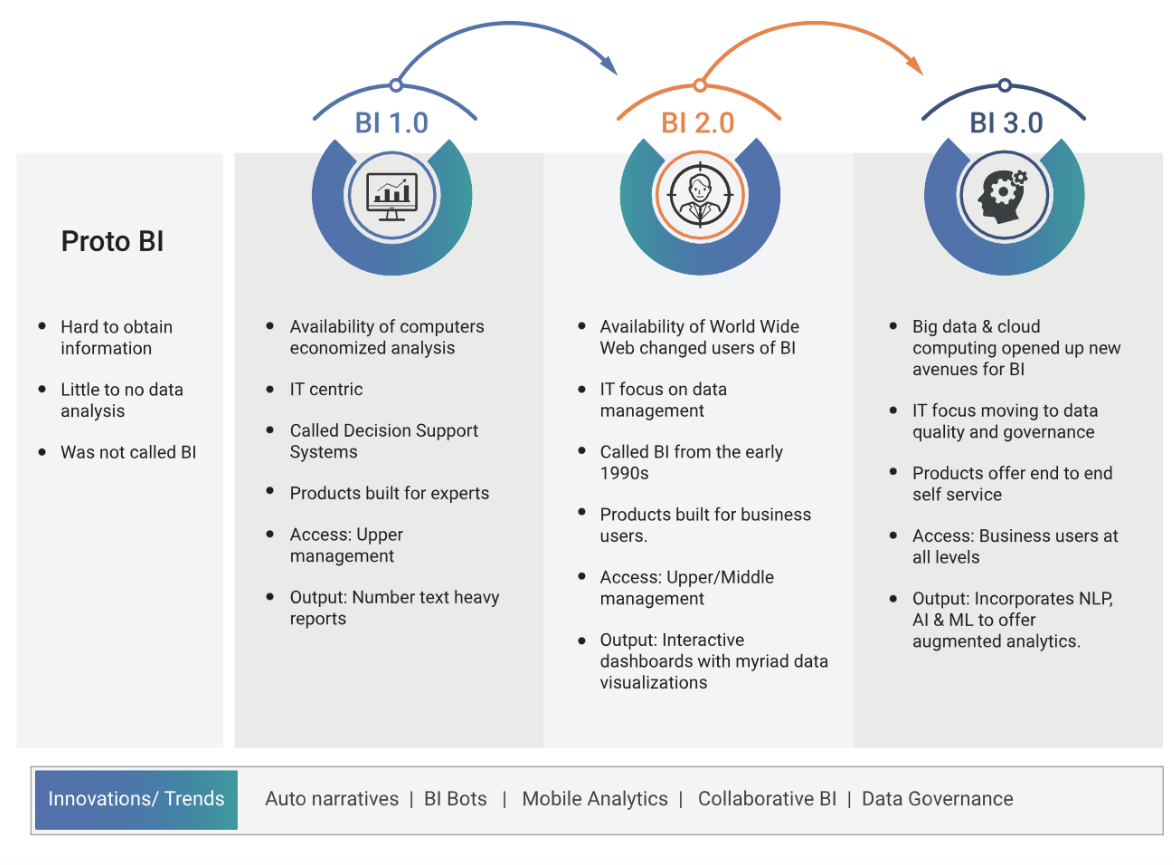
\includegraphics[height=0.75\textheight]{figures/evolution-business-intelligence.png}
            \caption{\tiny \url{https://www.agilisium.com/blogs/evolution-business-intelligence/}}
            \label{fig:evolution-of-business-intelligence}
        \end{figure}
    \end{frame}

    \begin{frame}
        \frametitle{Course Structure}
        The course is designed around the \alert{latest trends} in the field and comprises six modules:
        \begin{enumerate}
            \item Data ethics
            \item Natural language processing
            \item Guided learning and computational mathematics
            \item Semi- and unsupervised learning (clustering)
            \item Event analysis in processes (process mining)
            \item Capstone project
        \end{enumerate}
    \end{frame}

    \begin{frame}{Capstone Project}
        \begin{columns}
            \begin{column}{0.7\textwidth}
                The capstone project integrates the course's modules into a single, cohesive experience.
                Students will collaborate with \alert{Tixly Ticketing},
                employing their actual data to craft a comprehensive technical report and presentation.
                \newline\newline
                This pivotal project simulates a professional BI consultancy, emphasizing
                the practical application of analytical skills in a real-world business context.
            \end{column}
            \begin{column}{0.3\textwidth}
                
\includegraphics[width=\linewidth]{figures/company}
            \end{column}
        \end{columns}
    \end{frame}


    \begin{frame}
        \frametitle{Course Instructors}
        \begin{figure}
            \begin{minipage}[t]{0.3\textwidth}
                \centering
                
\includegraphics[width=\linewidth]{figures/hafsteinne}
                Hafsteinn Einarsson \\
                Assistant Professor, Computer Science \\
                \url{hafsteinne@hi.is}
            \end{minipage}
            \hfill
            \begin{minipage}[t]{0.3\textwidth}
                \centering
                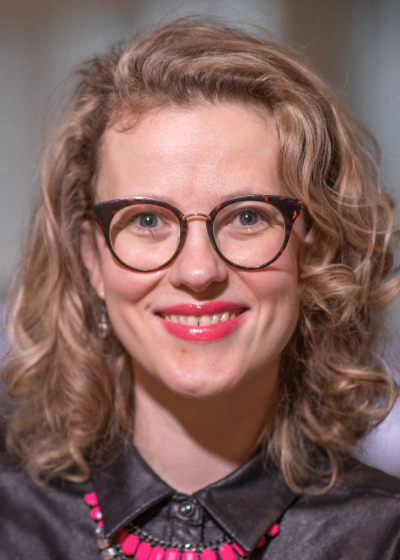
\includegraphics[width=\linewidth]{figures/helgaingim}
                Helga Ingimundardóttir \\
                Assistant Professor, Industrial Engineering
                \url{helgaingim@hi.is}
            \end{minipage}
            \hfill
            \begin{minipage}[t]{0.3\textwidth}
                \centering
                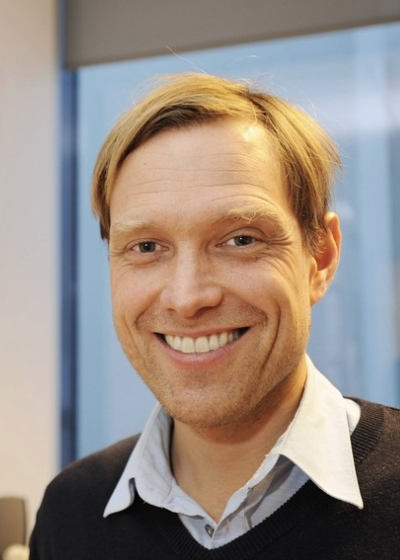
\includegraphics[width=\linewidth]{figures/hah}
                Henry Alexander Henrysson \\
                Research Specialist, Centre for Ethics \\
                \url{hah@hi.is}
            \end{minipage}
        \end{figure}

    \end{frame}

    \begin{frame}{Course Structure}
        \begin{table}
            \begin{tabular}{m{1.5cm} m{8cm} m{2.5cm}}
                \textbf{Week} & \textbf{Course Material}                      &                                                            \\\hline
                1-3           & Data ethics                                   & 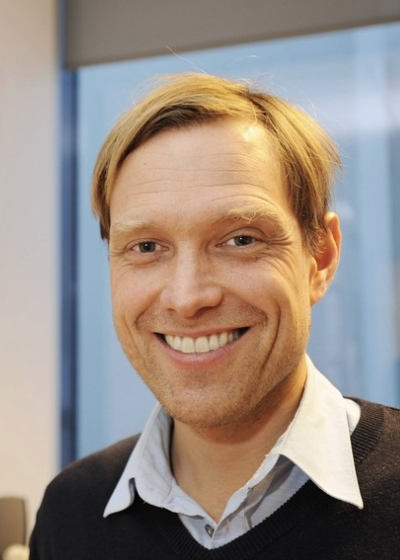
\includegraphics[height=.1\textheight]{figures/hah}        \\
                4-5           & Natural language processing                   & 
\includegraphics[height=.1\textheight]{figures/hafsteinne} \\
                6-7           & Guided learning and computational mathematics & 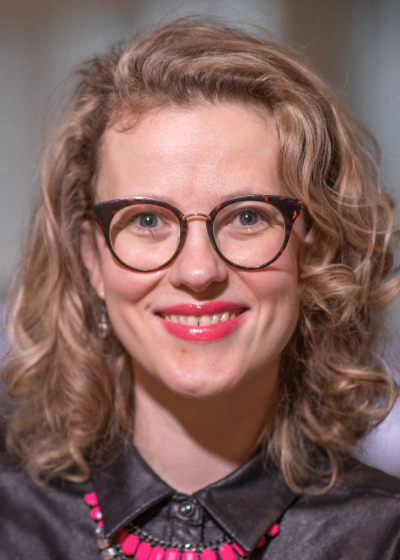
\includegraphics[height=.1\textheight]{figures/helgaingim} \\
                8-9           & Semi- and unsupervised learning (clustering)  & 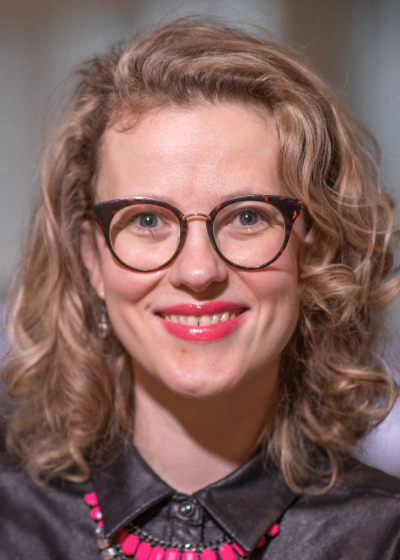
\includegraphics[height=.1\textheight]{figures/helgaingim} \\
                10-11         & Event analysis in processes (process mining)  & 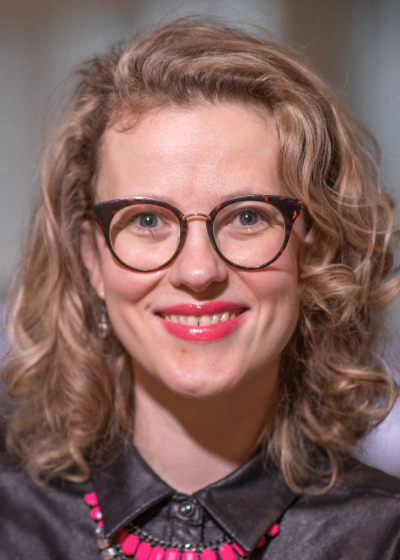
\includegraphics[height=.1\textheight]{figures/helgaingim} \\
                12-15         & Capstone Project (Easter Break included)      & 
\includegraphics[height=.1\textheight]{figures/company}    \\\hline
            \end{tabular}
        \end{table}
    \end{frame}

    \begin{frame}{Course Progression Flow}
        \begin{figure}
            \centering
            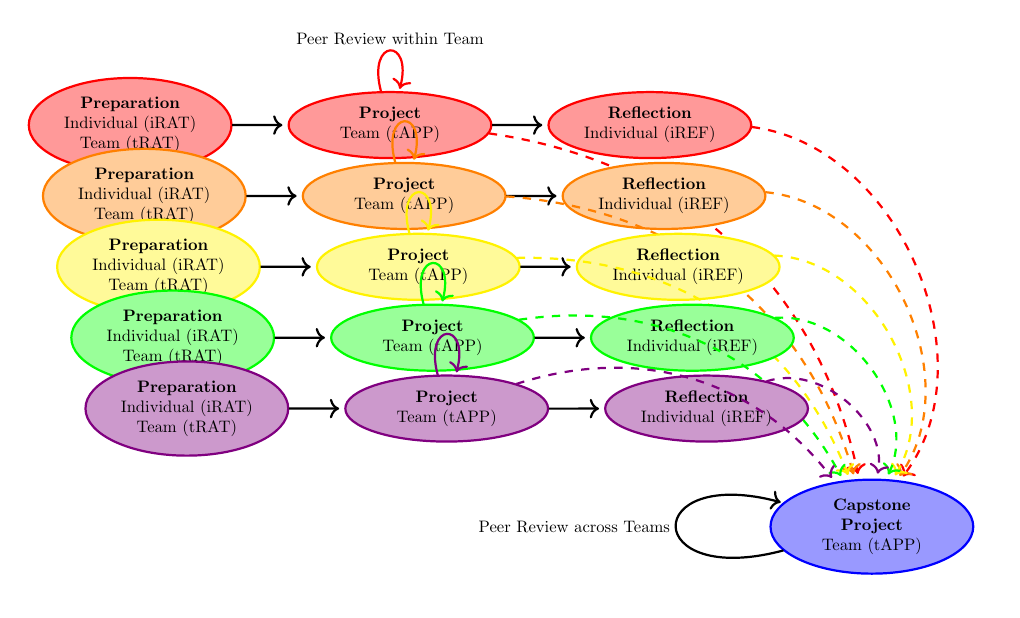
\begin{tikzpicture}
                [scale=0.6, transform shape,
                node distance=5.5cm,
                auto,
                block/.style={
                    ellipse,
                    draw,
                    thick,
                    fill=green!40,
                    text width=2.8cm,
                    align=center,
                    minimum height=1cm,
                    minimum width=3.0cm
                },
                line/.style={
                    draw, thick, ->, shorten >=2pt
                },
                dashedline/.style={
                    draw, thick, ->, dashed, shorten >=2pt
                },
                red/.style={block, draw=red, fill=red!40},
                orange/.style={block, draw=orange, fill=orange!40},
                yellow/.style={block, draw=yellow, fill=yellow!40},
                green/.style={block, draw=green, fill=green!40},
                violet/.style={block, draw=violet, fill=violet!40},
                blue/.style={block, draw=blue, fill=blue!40}
                ]

                % Capstone node
                \node[blue] (capstone) at (16cm,-10cm) {\textbf{Capstone Project}\\Team (tAPP)};
                % Circular arrow for capstone peer review
                \draw [line] (capstone) edge[loop left] node {Peer Review across Teams} (capstone);

                % Define positions for nodes
                \foreach \color/\pos in {red/1, orange/2, yellow/3, green/4, violet/5}{
                    \node[\color] (RAT\pos) at (\pos*.3cm,-\pos*1.5cm) {\textbf{Preparation}\\Individual (iRAT)\\
                    Team (tRAT)};
                    \node[\color, right of=RAT\pos] (APP\pos) {\textbf{Project}\\Team (tAPP)};
                    \node[\color, right of=APP\pos] (REF\pos) {\textbf{Reflection}\\Individual (iREF)};

                    % Edges
                    \path [line] (RAT\pos) -- (APP\pos);
                    \path [line] (APP\pos) -- (REF\pos);

                    % Circular arrow for peer review within team
                    % Conditional text for the loop
                    \ifnum\pos=1
                    \draw [line,draw=\color] (APP\pos) edge[loop above] node {\mbox{Peer Review within Team}} (APP\pos);
                    \else
                    \draw [line,draw=\color] (APP\pos) edge[loop above] (APP\pos);
                    \fi

                    % Connect APP nodes to Capstone with staggered entry points
                    \path [dashedline,draw=\color] (APP\pos) to[bend left=35] (capstone);

                    % Connect REF nodes to Capstone with staggered entry points
                    \path [dashedline,draw=\color] (REF\pos) to[bend left=60] (capstone);
                }
            \end{tikzpicture}
        \end{figure}
    \end{frame}

    \begin{frame}{Course Assessment}
        \begin{columns}[T] % align columns
            \begin{column}{.48\textwidth}
                \begin{block}{Modules (50\% Total)}
                    \begin{itemize}
                        \item Each Module: 10\%
                        \begin{itemize}
                            \item iRAT: 1\%
                            \item tRAT: 1\%
                            \item tAPP: 4\%
                            \item iREF: 4\%
                        \end{itemize}
                    \end{itemize}
                \end{block}
            \end{column}%
            \hfill%
            \begin{column}{.48\textwidth}
                \begin{block}{Capstone Project (50\% Total)}
                    \begin{itemize}
                        \item Peer Review - Feedback: 20\%
                        \begin{itemize}
                            \item Student Feedback: 10\%
                            \item Instructor Evaluation of Feedback: 10\%
                        \end{itemize}
                        \item Presentation: 20\%
                        \item Technical Report: 40\%
                        \item Company's Grade: 20\%
                    \end{itemize}
                \end{block}
            \end{column}%
        \end{columns}
    \end{frame}


\end{document}

